 
\section{Imaging and Tracking Payload Unit}

In the CDR examplary images for the design of the ITPU controller using a raspberryPi were used, but as stated there as well the BeagleBoard (BB) provides the processing capabilities and the interfaces in this project. In figure \ref{itpu_setup} the actual setup of the system can be seen. Figure \ref{fig:itpu_pcb} presents the top and bottom view of the produced and populated circuit board which was designed to be tightly stacked to the main header of the BB and hold in place by nylon screws.

\begin{figure}
\label{fig:itpu_pcb}
\begin{centering}
\subfloat[Top]{\begin{centering}
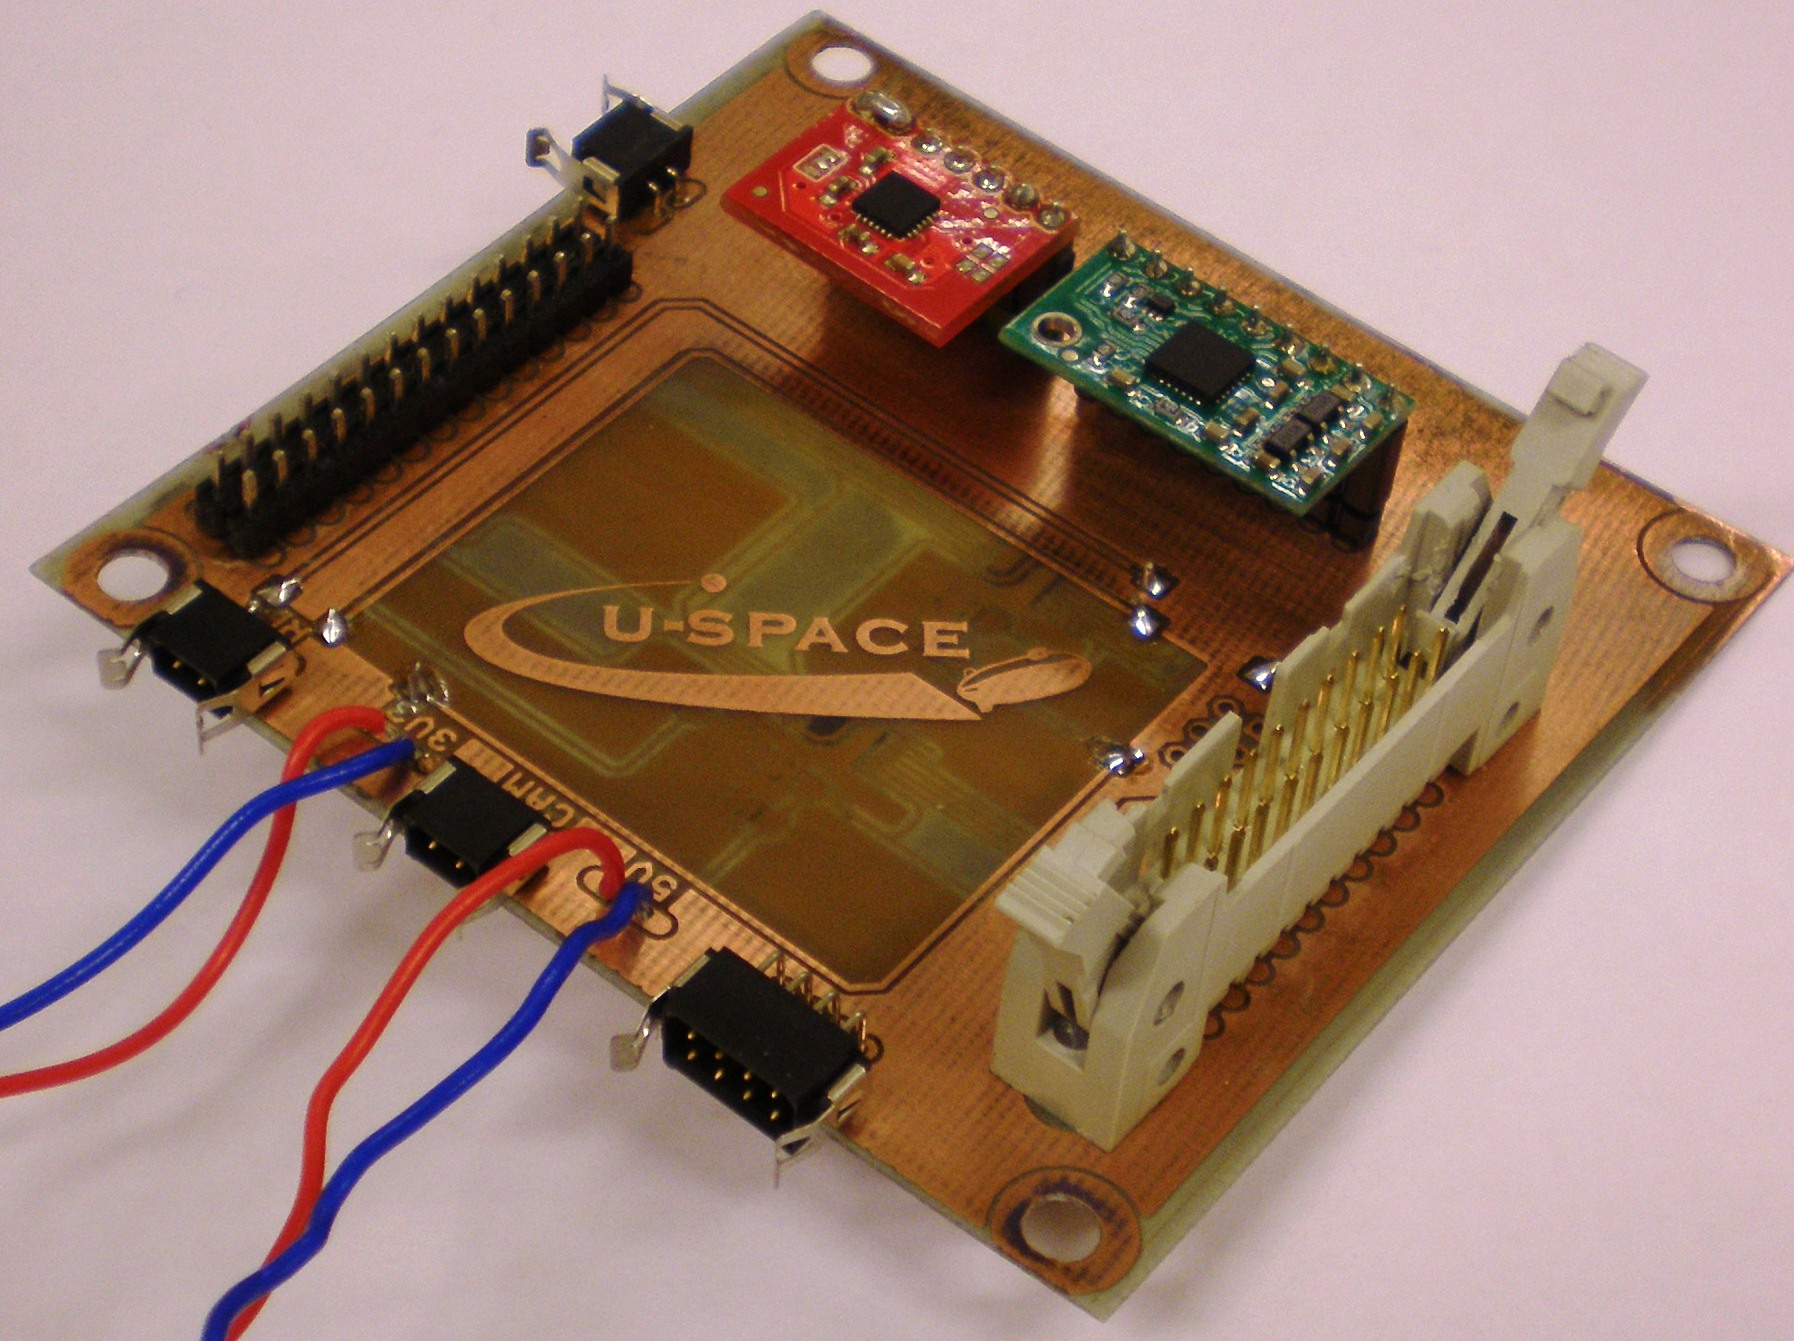
\includegraphics[height=0.25\textheight]{figures/LVC_top.JPG}
\par\end{centering}

}\subfloat[Bottom]{\begin{centering}
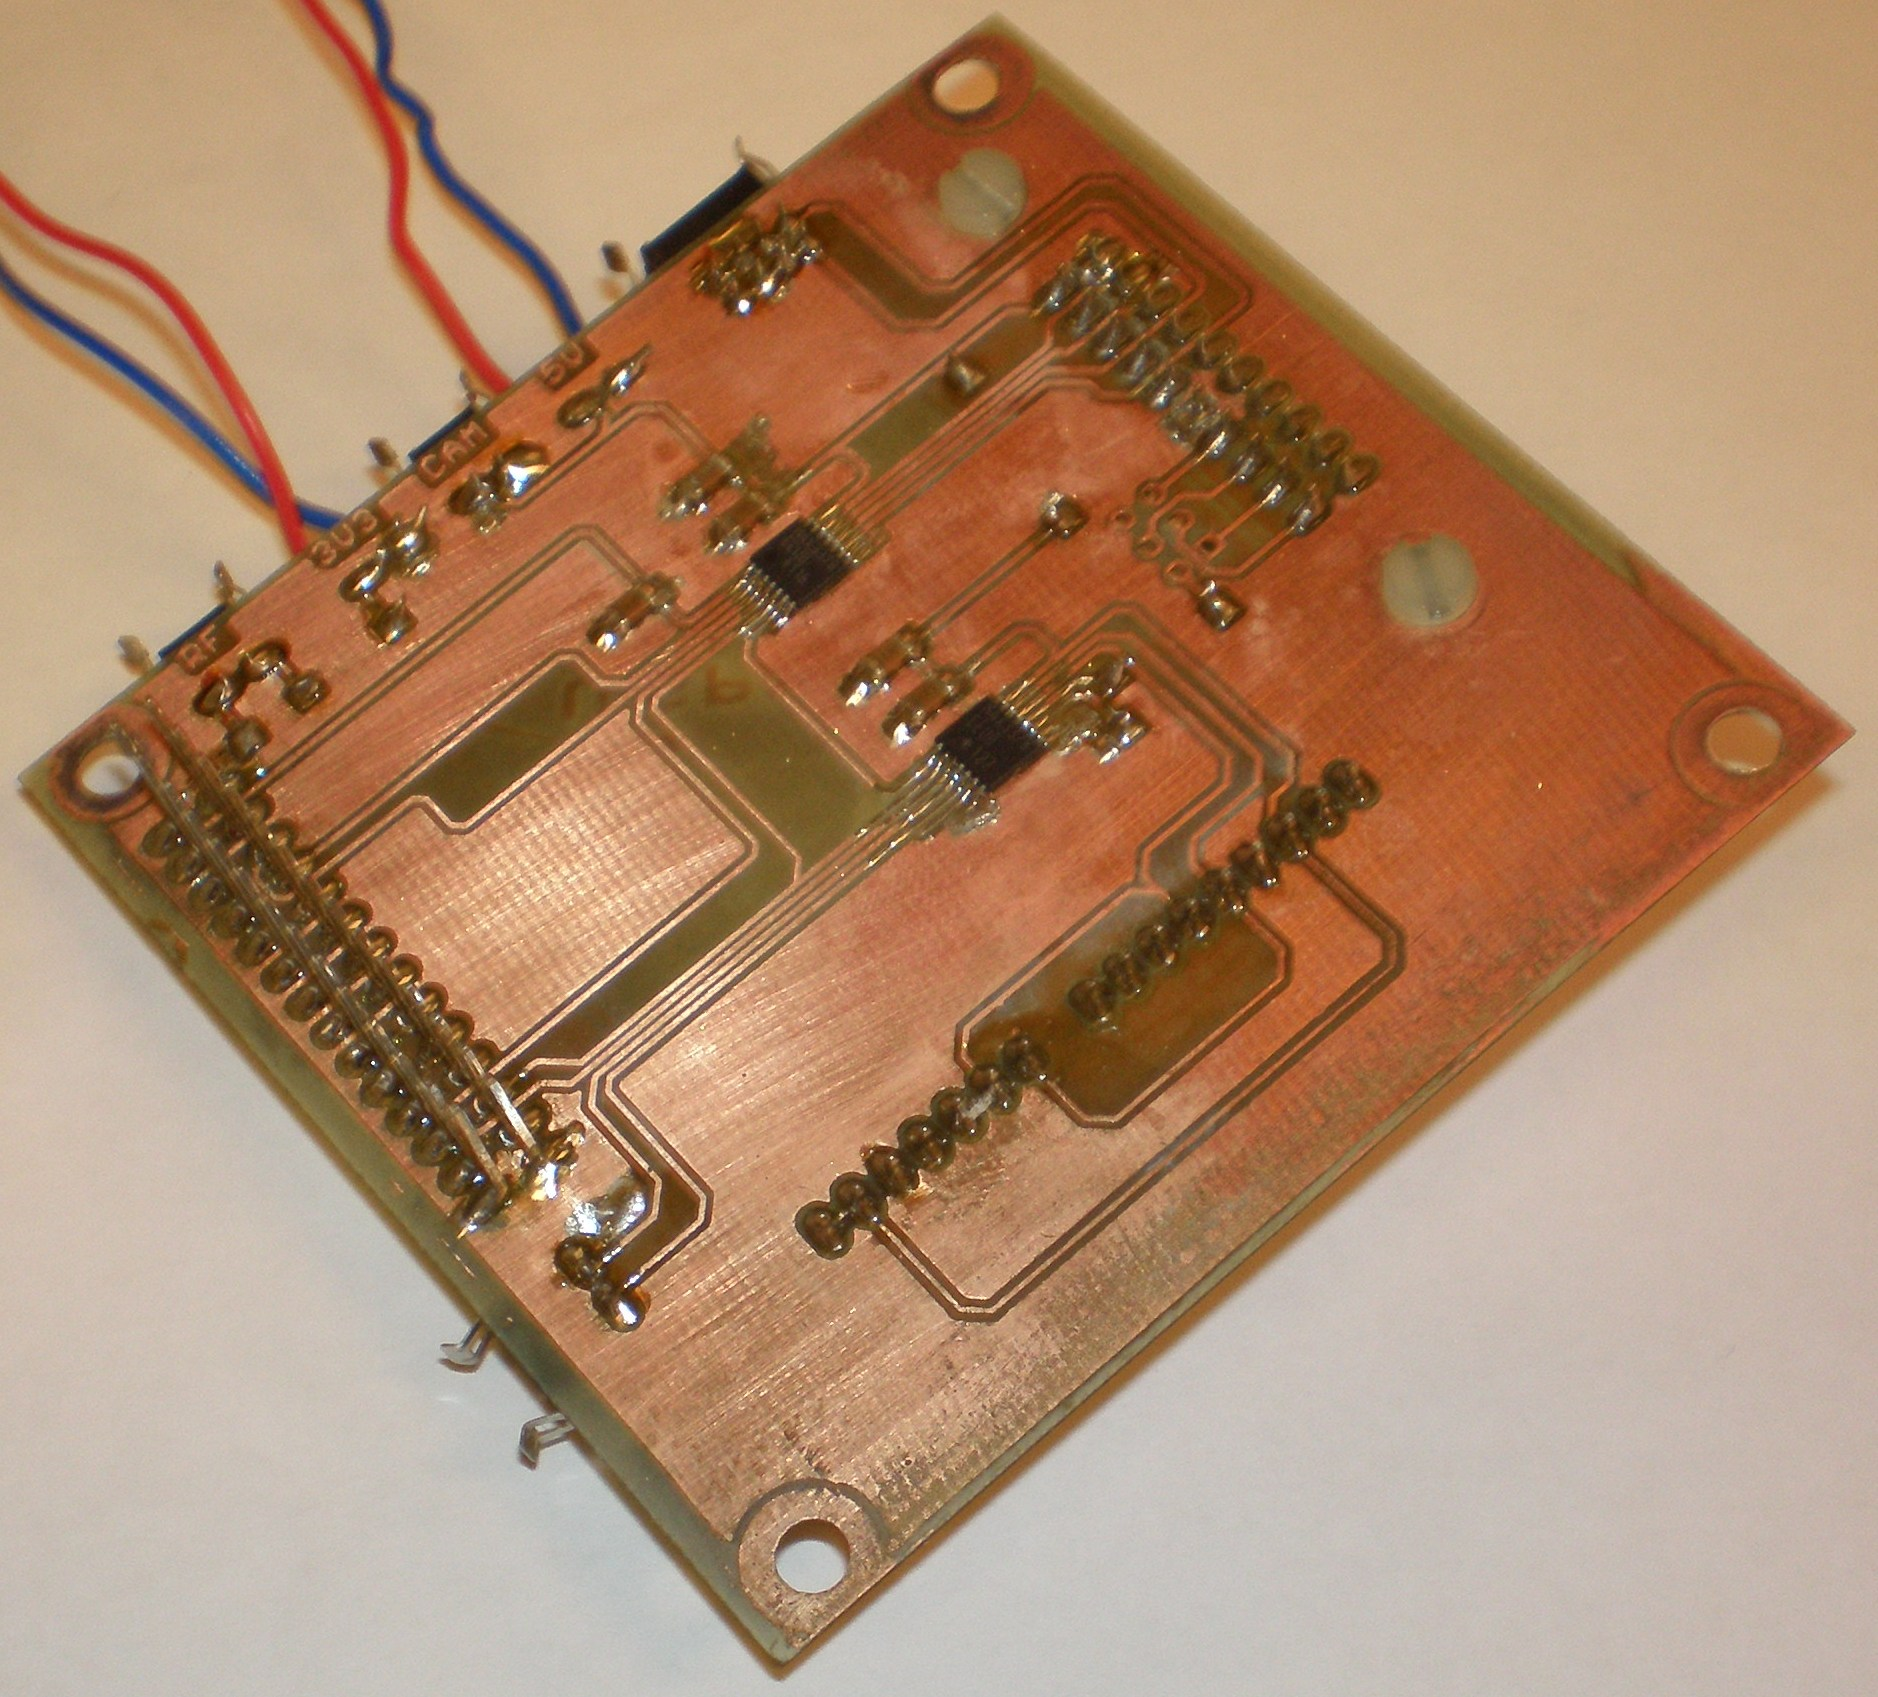
\includegraphics[height=0.25\textheight]{figures/LVC_bottom.JPG}
\par\end{centering}

}
\par\end{centering}
\caption{Populated expansion PCB of the ITPU}
\end{figure}

\begin{figure}
\label{fig:itpu_setup}
\begin{centering}
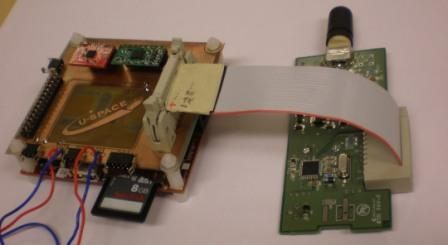
\includegraphics[height=0.25\textheight]{figures/itpu-setup.jpg}
\par\end{centering}
\caption{Setup of the ITPU consisting of the BeagleBoard, the E-Tag and the expansion board with sensors}
\end{figure}


One set of design changes were made for the inclusion of the communication and telemetry modules (see \ref{sec:com}). As the main expansion header of the BB only provides access to one set of UART pins which was used to communicate with the E-TAG gps module, another UART of the BB was muxed to the supplementary expansion header J4, converted to a 3.3~V level and connected to the X-Bee circuit board via wires. Initially the I2C interface was only planned to be converted from the 1.8~V level of the BB to the 3.3~V of the attitude sensors and vice versa. With the inclusion of the telemetry conversion module (see \ref{sec:telemetryConv}) it was necessary to also shift the level to 5~V to incorporate the ADCs. 

Both two sensor systems (attitude and telemetry measuring) worked stable seperately, but caused unstable behavior when operated in parallel on the same I2C-bus. As this was thought to be related to the multiple voltage level shifts it was tried to use an additional I2C-bus muxed to pins of the J4 and J5 expansion header of the BB, but the 2nd I2C-bus could not be activated on the BB rev.C4 used for the initial design.
On the software side the integration of the telemetry and communication system together with the attitude determination and imaging system needed only minor additions to the code base to provide interfaces for communication between both systems. 

A major drawback and cause for big changes compared to the CDR was the sudden failure of the BB between the pre-flight test and the scheduled flight-test. As no replacement board of the same kind could be aquired on such a short notice a provided BB-xM was made to fit into the already designed and build system. Although the BB-xM is in general pin-compatible to the BB (rev.C4), the main problem was the direction of the main expansion header. For the BB of the initial design the~(female) header was mounted on the top side of the BB, hence the ITPU-pcb was designed to be directly stacked on top of the BB. In contrast, the expansion header of the BB-xM was mounted to the bottom side of the BB-xM. Therefore a direct connection between both boards was not possible anymore and a produced ribbon cable had to be used which could not provide a fully stable connection between the BB-xM and the expansion board. However on the BB-xM it was possible to enable the second I2C-bus on the J4 and J5 expansion headers.
